Recent years have seen a rapid increase of robotic deployment, beyond traditional applications in cordoned-off workcells in factories, into new, more collaborative use-cases. For example, social robotics and service robotics have targeted scenarios like rehabilitation, where a robot operates in close proximity to a human. Where industrial applications envision full autonomy, these collaborative scenarios will always involve interaction between the robotic systems and humans. Thus, these scenarios require effective communication between robots and people.

When the robot's form permits, researchers can design such interactions using principles informed by research on embodied face-to-face human--human communication.  In particular, by realizing \emph{pointing gestures}, an articulated robotic arm with a directional end-effector can exploit a fundamental ingredient of human communication \cite{kita2003pointing}.  Thus far, roboticists have primarily researched pointing gestures that identify objects in simple settings \cite[a.o.]{han2018placing,holladay2014legible,zhao2016experimental}.  Human pointing exhibits richer and more diverse interpretations \cite{kendon:2004}.  This paper develops an empirically-grounded approach to robotic pointing that covers a wider range of physical settings, task contexts and communicative goals.

Our work has two contributions.  First, we create a systematic dataset, involving over 7000 human judgments, where crowd workers describe their interpretation of animations where simulated robots instruct pick-and-place tasks.  Planned comparisons allow us to compare pointing actions that identify objects (referential pointing) with those that identify locations (spatial pointing), and allow us to quantify the effect of accompanying speech, task constraints and scene complexity, as well as variation in the spatial content the scene.  This new resource documents important differences in the way pointing is interpreted in different cases for the first time.  For example, referential pointing is typically robust to the exactness of the pointing gesture, whereas spatial pointing is much more sensitive and requires more deliberate pointing to ensure a correct interpretation.  The Experiment Design section explains the different conditions we explore, the power analysis for our preregistered protocol and the process of data collection. 

\begin{figure}[t]
    \centering
    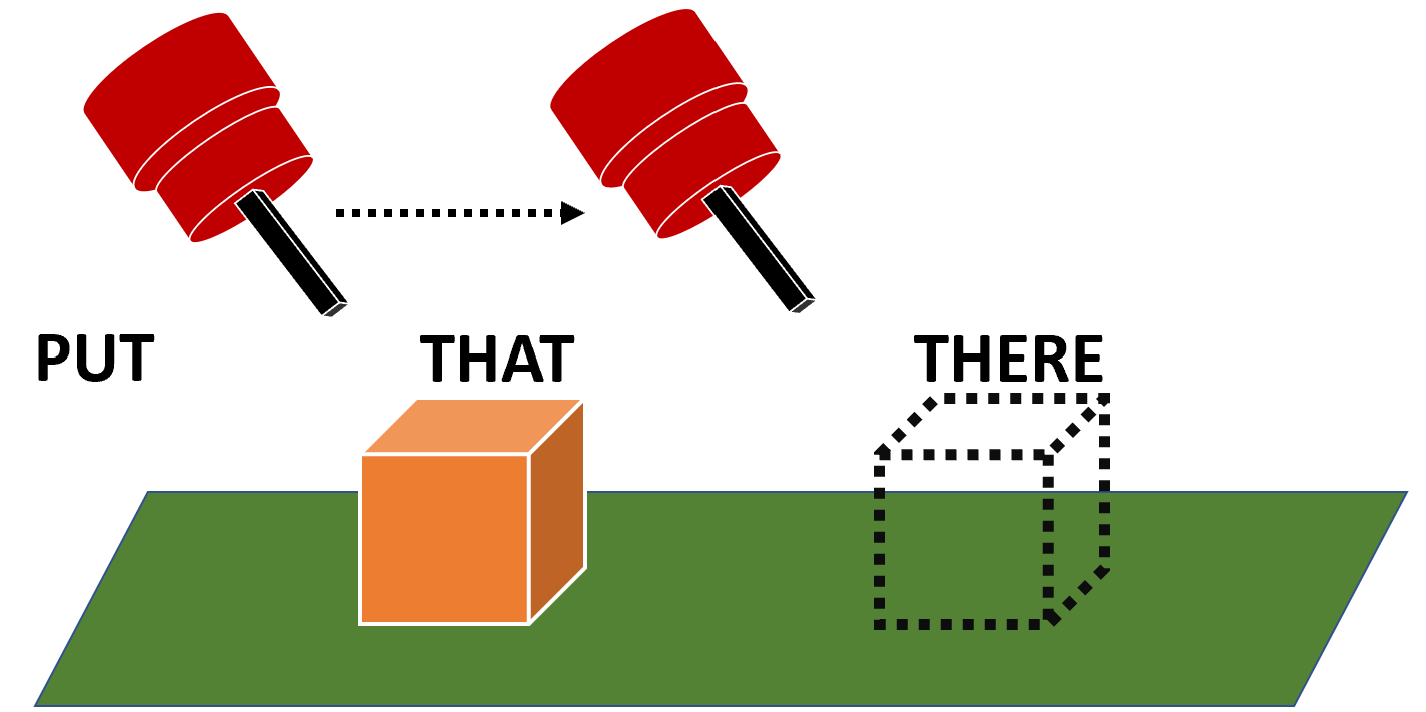
\includegraphics[width=0.4\textwidth, trim={0 0.3in 0 0in},clip]{figures/putthatthere2.png}
    \caption{A pick-and-place task requires a \textit{referential} pointing action to the object (orange cube) at the initial position, and a \textit{spatial} pointing action to a final placement position (dotted cube). Such an action by a robot (in red) can also be accompanied by verbal cues like \textit{"Put that there."}}
    \label{fig:pap}
\end{figure}

Our second contribution is a set of interpretive principles, inspired by the literature on vague communication, that summarize our findings about robot pointing.  Our results suggest that pointing selects from a set of candidate interpretations determined by the type of information specified, the possibilities presented by the scene, and the options compatible with the current task.  In particular, we propose that pointing picks out all candidates that are not significantly further from the pointing ray than the closest alternatives.  Based on our empirical results, we present design principles that formalize the relevant notions of ``available alternatives'' and ``significantly further away'' and can be used in implementing future pointing robots.  The Analysis and Design Principles sections explains and justifies this approach and contextualizes it with previous research.

% \begin{hyp}
% In the domain of communication of between a robot and a human observer referential pointing is dependent on the contextual cues and is robust to the exactness of the pointing gesture, whereas the spatial pointing is far more sensitive, and requires more deliberate pointing for ensuring a correct interpretation.
% \end{hyp}




